\chapter{Aspectos Básicos de las Estadísticas}
\subsection*{Concepto de la Estadística}
Es una ciencia que proporciona un conjunto de métodos y técnicas que permiten recolectar, clasificar, organizar, analizar y presentar datos de forma adecuada para tomar decisiones frente a una incertidumbre o describir o afirmar algo acerca de la población. Esta definición permite clasificar la Estadística en: Estadística \textbf{Descriptiva} y Estadística \textbf{Inferencial}.
\subsubsection*{Estadística Descriptiva}
Es la parte de la Estadística que proporciona un conjunto de métodos, con el fin de describir o analizar datos.
\subsubsection*{Estadística Inferencial}
\section{Conceptos Generales de la Estadística}
\subsection{Generalidades}
\begin{enumerate}[label=(\roman*)]

\item \textbf{Población:} Es el conjunto o totalidad de elementos, sean personas, objetos o cosas que presentan uno o más características que nos interesan acerca de las cuales intentamos obtener conclusiones.

\item \textbf{Tamaño de la Población:} Número de elementos de la población, denotado usualmente por: $N$. 

\item \textbf{Muestra: } Es parte o subconjunto de la población.

\item \textbf{Tamaño de la Muestra: } Cantidad de elementos de la Muestra. Denotado por: $n$.

\item \textbf{Parámetro:} Es una medida numérica que describe una característica de la población. Los parámetros mas usados de la población son:
\begin{itemize}
\item Media Poblacional ($\mu$)$^\ast$\blfootnote{Todos los puntos marcados con un $^\ast$ serán explicados mas adelante, o puedes ver el índice}
\item Varianza Poblacional ($\sigma^2$)$^\ast$
\item Desviación Estándar Poblacional ($\sigma$)$^\ast$
\item Proporción Poblacional ($\pi$ ó $p$)$^\ast$
\end{itemize}
\item \textbf{Estadígrafos:} Es una medida numérica que describe una característica de la muestra. Los estadígrafos mas usados son:
\begin{itemize}
\item Media Muestral ($\bar{x},\bar{y}$)$^\ast$
\item Varianza Muestral ($S^2,\hat{S}^2$)$^\ast$
\item Desviación Estándar ($S,\hat{S}$)$^\ast$
\item Proporción Muestral ($\hat{\pi}$ ó $\hat{p}$)$^\ast$
\end{itemize}
\end{enumerate}

\subsection{Variables Estadísticas}
Se denomina variable estadística a la característica o combinación de características de una población:
\subsubsection{Tipos de Variables Estadísticas}
Están clasificadas de la siguiente manera:
\begin{itemize}
\item \textbf{Cualitativas:}
\begin{itemize}
\item \textbf{Variables Nominales:} Es aquella cuyo valor se expresa en categorías sin ningún tipo de orden o clasificación.
\item \textbf{Variables Ordinales:} Es aquella cuyo valor se expresa en categorías pero se busca una clasificación de orden.
\end{itemize}
\item \textbf{Cuantitativas:}
\begin{itemize}
\item \textbf{Variables Discretas:} Se dice cuando es resultado de la operación de contar.
\item \textbf{Variables Continuas:} Una variable es continua cuando se encuentra por medición o comparación, y es expresada por cualquier número real. 
\end{itemize}
\end{itemize}

\begin{figure}[h]
\begin{tabular}{|p{3.5cm}|p{3.5cm}|p{3.5cm}|p{3.5cm}|}
\hline 
\textbf{Nominales} & \textbf{Ordinales} & \textbf{Discretas} & \textbf{Continuas} \\ 
\hline 
Sexo & Tamaño & Número de Hijos & Edad \\ 
\hline 
Nacionalidad & Grado de Instrucción  & Número de Alumnos & Estatura \\ 
\hline 
Color & Categoría  & Número de Accidentes & Peso \\ 
\hline 
\end{tabular} 
\caption{Tabla con algunos ejemplos de los tipos de Variables}
\end{figure}

\section{Representación de la Información en Cuadros o Tablas}
Para entender como hacer tablas Estadísticas y Representaciones Gráficas, hay ciertos conceptos que es necesario conocer antes:
\subsection{Conceptos Iniciales}
\begin{enumerate}[label=(\roman*)]
\item \textbf{Clase:} Es el conjunto de observaciones cualitativas o cuantitativamente iguales o muy próximas.
\item \textbf{Límite de Clase:} Son los valores de las observaciones, mínimo y máximo que pueden tener los datos, incluidos en la \textit{Clase.}
\item \textbf{Intervalo de Clase:} Es la distancia entre los límites de la \textit{Clase} expresados de la siguiente manera:
$$y_{i-1}'  y_i'$$
\item \textbf{Marca de Clase:} Es el punto medio de cada uno de los intervalos. Si es constante se puede expresar como $c_j$, caso contrario $y_i$. Se tiene la siguiente fórmula para calcularlo:
$$c_j = \dfrac{y_{i-1}'+y_i'}{2}$$
\item \textbf{Recorrido de la Variable:} Es el valor de la diferencia entre los límites de los datos de la muestra (el máximo y el mínimo), está representado por: $R$.
\begin{itemize}
\item \textbf{Datos No Agrupados\footnote{También llamados \textbf{Datos Originales}}:} $R=y_k-y_i$
\item \textbf{Datos Agrupados:} $R=y_k'-y_i'$
\end{itemize}
\item \textbf{Amplitud de Intervalo:} Expresado por $C$ y $C_i$, para cuando es constante y variable respectivamente.
$$C_i = y_i' - y_{i-1}'$$
\item \textbf{Número de Intervalos:} $$k=\dfrac{R}{C_i}$$
\end{enumerate}
\subsection{Frecuencia}
Es la cantidad de Observaciones incluidas en una clase.
\subsubsection{Frecuencias}
\begin{enumerate}[label=(\roman*)]
\item \textbf{Frecuencia Absoluta Simple $(f_i)$:} es el numero de veces que se repite cada observación.
\item \textbf{Frecuencia Absoluta Acumulada $(F_i)$:} Expresado como:
$$F_i = \sum_{j=1}^{i}f_j$$
\item \textbf{Frecuencia Relativa Simple $(h_i)$:} $$h_j=\dfrac{f_j}{n}$$
\item \textbf{Frecuencia Relativa Acumulada $(H_i)$:} $$H_i=\dfrac{F_i}{n}=\sum_{j=1}^{i}h_j$$
\end{enumerate}

\subsubsection{Propiedades de la Frecuencias}
\begin{itemize}
\item $f_1+f_2+f_3+\ldots + f_k = \displaystyle\sum_{i=1}^{k} f_i=n$
\item $h_1+h_2+h_3+\ldots + h_k = \displaystyle\sum_{i=1}^{k} h_i=1$
\item $\forall i \in I, $
$\begin{cases} 
0\leq h_i \leq 1\\
0 \leq f_i \leq n
 \end{cases}$
\item $f_1=F_1 \leq F_2 \leq F_3 \leq \cdots \leq F_k=n$
\item $h_1 = H_1 \leq H_2 \leq H_3 \leq \cdots \leq H_k = 1$ 
\item $H_j = H_{j-1}+h_j$
\item $F_j = F_{j-1}+f_j$
\end{itemize}

\subsection{Tablas de Distribución de Frecuencia}
\subsubsection{Distribución de Frecuencia para Datos Agrupados no en Intervalos de Clase}
\begin{center}
\begin{tabular}{|C{1.5cm}|C{1.5cm}|C{1.5cm}|C{1.5cm}|C{1.5cm}|}
\hline
$x_i$ & $f_i$ & $F_i$ & $h_i$ & $H_i$\\ \hline
$x_1$ & $f_1$ & $F_1$ & $h_1$ & $H_1$\\ \hline
$x_2$ & $f_2$ & $F_2$ & $h_2$ & $H_2$\\ \hline
$x_3$ & $f_3$ & $F_3$ & $h_3$ & $H_3$\\ \hline
$\vdots$ & $\vdots$ & $\vdots$ & $\vdots$ & $\vdots$ \\ \hline
$x_k$ & $f_k$ & $F_k=n$ & $h_k$ & $H_k=1$ \\ \hline
$Totales$ & $n$ &  & $1$ & \\ 
\hline
\end{tabular}
\end{center}
\subsubsection{Distribución de Frecuencias para Datos Agrupados en Intervalo de Clase}
\begin{center}
\begin{tabular}{|C{1.5cm}|C{1.5cm}|C{1.5cm}|C{1.5cm}|C{1.5cm}|}
\hline
$y_{i-1}'-y_i'$ & $f_i$ & $F_i$ & $h_i$ & $H_i$\\ \hline
$y_0'-y_1'$ & $f_1$ & $F_1$ & $h_1$ & $H_1$\\ \hline
$y_1'-y_2'$ & $f_2$ & $F_2$ & $h_2$ & $H_2$\\ \hline
$y_2'-y_3'$ & $f_3$ & $F_3$ & $h_3$ & $H_3$\\ \hline
$\vdots$ & $\vdots$ & $\vdots$ & $\vdots$ & $\vdots$ \\ \hline
$y_{k-1}'-y_k'$ & $f_k$ & $F_k=n$ & $h_k$ & $H_k=1$ \\ \hline
$Totales$ & $n$ &  & $1$ & \\ 
\hline
\end{tabular}
\end{center}
\subsubsection{Estructura de una Tabla Estadística}
\begin{enumerate}
\item \textbf{Título}
\item \textbf{Cuerpo Propiamente }
\begin{itemize}
\item Encabezamiento
\item Cuerpo
\item Columna Matriz
\end{itemize}
\item \textbf{Indicadores Complementarios}
\begin{itemize}
\item Fuente(s)
\item Nota(s)
\item Comentarios
\end{itemize}
\end{enumerate}
\section{Representaciones Gráficas}
Las gráficas son instrumentos estadísticos muy útiles para dar idea global acerca de una situación estadística:
\subsection{Diagrama de Barras}
\pgfplotstableread[row sep=\\,col sep=&]{
    interval & carT & carD & carR \\
    0     & 1.2  & 0.1  & 0.2  \\
    2     & 12.8 & 3.8  & 4.9  \\
    4    & 15.5 & 10.4 & 13.4 \\
    6   & 14.0 & 17.3 & 22.2 \\
    8  & 7.9  & 21.1 & 27.0 \\
    10      & 3.0  & 22.3 & 28.6 \\
    }\mydata
\begin{center}
\begin{tikzpicture}
    \begin{axis}[
            ybar,
            symbolic x coords={0,2,4,6,8,10},
            xtick=data,
        ]
        \addplot[fill=lightgray,line width=0.75pt] table[x=interval,y=carT]{\mydata};
    \end{axis}
\end{tikzpicture}
\end{center}
\subsection{Diagrama de Sectores}

\subfile{Imagenes/DiagramaSectores}


\subsection{Diagrama de Bastones}
\begin{center}
\begin{tikzpicture} 
\begin{axis} 
\addplot[ycomb,draw=black,fill=black,line width=1pt] plot coordinates {(0,3) (1,2) (2,4) (3,1) (4,2)}; 
\addplot [only marks] table {
0 3
1 2
2 4
3 1
4 2
};
\end{axis} 
\end{tikzpicture}
\end{center}
\subsection{Histograma y Polígono de Frecuencia}
\begin{center}
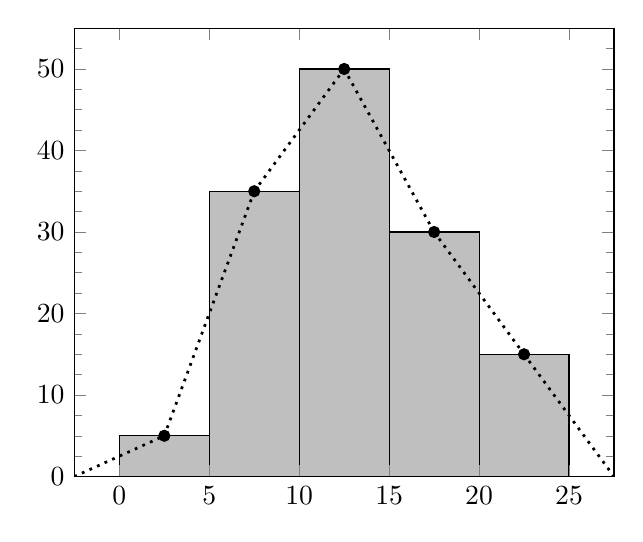
\begin{tikzpicture}
\begin{axis}[
    ymin=0, ymax=55,
    minor y tick num = 3,
    area style,
    ]
\addplot+[ybar interval,mark=no,fill=lightgray, draw=black] plot coordinates { (0, 5) (5, 35) (10, 50) (15, 30) (20, 15) (25, 0) };
\addplot [only marks] table {
2.5 5
7.5 35
12.5 50
17.5 30
22.5 15
};
\draw[dotted,line width=1pt] (-2.5,0) -- (2.5,5);
\draw[dotted,line width=1pt] (2.5,5) -- (7.5,35);
\draw[dotted,line width=1pt] (7.5,35) -- (12.5,50);
\draw[dotted,line width=1pt] (12.5,50) -- (17.5,30);
\draw[dotted,line width=1pt] (17.5,30) -- (22.5,15);
\draw[dotted,line width=1pt] (22.5,15) -- (27.5,0);
\end{axis}
\end{tikzpicture}
\end{center}